% MA211 - Lecture 17
\documentclass[pdftex, xcolor=pdftex, dvipsnames,handout]{beamer}

\usetheme{MA211}
\usepackage{thumbpdf}
\usepackage{wasysym}
%\usepackage{ucs}
\usepackage[utf8]{inputenc}
\usepackage{pgf,pgfarrows,pgfnodes,pgfautomata,pgfheaps,pgfshade}
\usepackage{verbatim}

\usepackage{eurosym}
\usepackage{euler}

\usepackage{calc}               % Simple computations with LaTeX variables
%\usepackage[hang]{caption2}     % Improved captions

\usepackage{graphicx}           % Standard graphics package

\usepackage{amsmath, amsthm, amssymb}


\newcommand{\fquad}{\mbox{\qquad}}
\newcommand{\bull}{$\bullet$ }

\newcommand {\I} {\mathcal I}
\newcommand {\calI} {\mathcal I}
\def\disint{\displaystyle\int}

\DeclareMathOperator{\D}{d}
\newcommand{\dydx}{\frac{\D y}{\D x}}

%\definecolor{gray}{rgb}{0.69, 0.69, 0.69} \newcommand{\gray}[1]{\textcolor{gray}{#1}}
\definecolor{dogreen}{rgb}{0.33, 0.42, 0.18} \newcommand{\dogreen}[1]{\textcolor{dogreen}{#1}}
\definecolor{maroon}{rgb}{.5,0.2,0.2}\newcommand{\maroon}[1]{\textcolor{maroon}{#1}}
\definecolor{greena}{rgb}{.1,0.581,0.1}\newcommand{\greena}[1]{\textcolor{greena}{#1}}

\definecolor{blue4}{rgb}{0,0,.545}
\newcommand{\Blue}[1]{\textcolor{blue}{#1}}
\newcommand{\Red}[1]{\textcolor{red}{#1}}
\definecolor{pink}{rgb}{1.,0.75,0.8}
\definecolor{darkred}{rgb}{0.5,0.0,0.0}
\definecolor{darkgreen}{rgb}{0,0.3,0.3}
\definecolor{purple}{rgb}{0,0.3,0.3}
\definecolor{darkblue}{rgb}{0.0, 0.0, .5}
\definecolor{dpurple}{rgb}{.3,.0,.3}
\newcommand{\Green}[1]{\textcolor{darkgreen}{#1}}
\newcommand{\DRed}[1]{\textcolor{darkred}{#1}}
\newcommand{\DBlue}[1]{\textcolor{darkblue}{#1}}
\newcommand{\Purple}[1]{\textcolor{dpurple}{#1}}
\newcommand{\Emph}[1]{\textcolor{darkred}{\textbf{\it #1}}}
\newcommand{\remph}[1]{\textcolor{darkred}{\textbf{\emph{#1}}}}
\newcommand{\bemph}[1]{\textcolor{darkblue}{\textbf{\emph{#1}}}}
\newcommand{\gemph}[1]{\textcolor{darkgreen}{\textbf{\emph{#1}}}}
\newcommand{\Bf}[1]{\textcolor{darkblue}{\textbf{#1}}}
\newcommand{\Gf}[1]{\textcolor{darkgreen}{\textbf{#1}}}
\newcommand{\Rf}[1]{\textcolor{red}{\textbf{#1}}}
\newcommand{\Rmf}[1]{\textcolor{red}{\mathbf{#1}}}

\newcommand{\Conj}[1]{\overline{#1}}

\newcommand{\code}[1]{\textcolor{darkblue}{\texttt{\textbf{#1}}}}
\newcommand{\icode}[1]{{\blue\texttt{\textbf{\emph{#1}}}}}
\newcommand{\gcode}[1]{{\Green{\texttt{\textbf{\emph{#1}}}}}}
\newcommand{\out}[1]{\texttt{\emph{\textbf{\Green{#1}}}}}





\newenvironment{vminipage}%
{\begin{Sbox}\begin{minipage}\begin{small}\begin{verbatim}}%
{\end{verbatim}\end{small}\end{minipage}\end{Sbox}\fbox{\TheSbox}}

\newenvironment{nminipage}%
{\begin{Sbox}\begin{minipage}}%
{\end{minipage}\end{Sbox}\fbox{\TheSbox}}


\let\Arg\relax\DeclareMathOperator{\Arg}{\mathtt{Arg}}
\let\Arg\relax\DeclareMathOperator{\e}{\mathtt{e}}

\newcommand {\AND} {\wedge}
\newcommand {\OR} {\vee}
\newcommand {\NOT} {\neg}
\newcommand {\IMPLIES} {\rightarrow}
%\newcommand {\IFF} {\leftrightarrow}
\renewcommand {\iff} {\Leftrightarrow}
\newcommand {\NAND} {\uparrow}
\newcommand {\NOR} {\downarrow}
\newcommand {\XOR} {\otimes}

\newenvironment{citemize}% Colour items
{\begin{description}}%
{\end{description}}

\newcommand {\maroonitem}{\item[\maroon{$\bullet$}]}

\newcommand {\gitem} {\item {\includegraphics[width=.4cm,angle=-10]{img/green-bullet-on-white.ps}}}
\newcommand {\ritem} {\item {\includegraphics[width=.4cm,angle=-10]{img/red-bullet-on-white.ps}}}
\newcommand {\yitem} {\item {\includegraphics[width=.4cm,angle=-10]{img/yellow-bullet-on-white.ps}}}
\newcommand {\bitem} {\item {\includegraphics[width=.4cm,angle=-10]{img/blue-bullet-on-white.ps}}}

\newcommand {\greenitem} {\item {\includegraphics[width=.4cm,angle=-10]{img/green-bullet-on-white.ps}}}
\newcommand {\reditem} {\item {\includegraphics[width=.4cm,angle=-10]{img/red-bullet-on-white.ps}}}
\newcommand {\yellowitem} {\item {\includegraphics[width=.4cm,angle=-10]{img/yellow-bullet-on-white.ps}}}
\newcommand {\blueitem} {\item {\includegraphics[width=.4cm,angle=-10]{img/blue-bullet-on-white.ps}}}

\newcommand {\eq}[1]%
  {$\DBlue{#1}$}
\newcommand {\eqd}[1]%
  {$\displaystyle\DBlue{#1}$}
%\newcommand{\eq}[1]{\boldmath \DBlue{$#1$}}


\newcommand {\csf}{\centerslidesfalse}
\newcommand {\cst}{\centerslidestrue}

\newcommand {\vecii}[2] {   \big(\begin{smallmatrix} #1 \\ #2 \end{smallmatrix}\big)}
\newcommand{\atwo}[2]{\left(\!\!\begin{array}{c} #1 \\ #2 \end{array}\!\!\right)}


\newcommand{\C}{\mathbb{C}}
\newcommand{\Q}{\mathbb{Q}}
\newcommand{\R}{\mathbb{R}}
\newcommand{\N}{\mathbb{N}}
\newcommand{\Z}{\protect\mathbb{Z}}  % protect for index.
\newcommand {\Rs}{ \mathbb{R}}
\newcommand {\Cs}{ \mathbb{C}}
\newcommand {\Rnn}{ \mathbb{R}^{n \times n}}
\newcommand {\Rn}{ \mathbb{R}^{n}}


\newcommand{\mblock}{%
\setbeamercolor*{block title}{bg=maroon,fg=white}
\setbeamercolor*{block body}{bg=white,fg=maroon}
}%

\newcommand{\bblock}{%
\setbeamercolor*{block title}{bg=Steel,fg=white}
\setbeamercolor*{block body}{bg=Mylightgray,fg=Steel}
}%

\newcommand{\gblock}{%
\setbeamercolor*{block title}{bg=Green,fg=white}
\setbeamercolor*{block body}{bg=Mylightgray,fg=darkgreen}
}%


\newcommand{\rblock}{%
\setbeamercolor*{block title}{bg=Red,fg=white}
\setbeamercolor*{block body}{bg=white,fg=Black}
}%


\newcommand{\TakeNotes}{
\includegraphics[width=2cm]{TakeNote}}

\def\eps{\varepsilon}
\newcommand {\del}[2]{ {\frac{\partial #1}{\partial #2}}}
\newcommand {\x}[1]{x^{[#1]}}
\newcommand {\delx}{ {\frac{\partial}{\partial x}}}
\newcommand {\delt}{ {\frac{\partial}{\partial t}}}
\newcommand {\dely}{ {\frac{\partial}{\partial y}}}
\newcommand {\ith}{{(i)}}
\renewcommand {\vec}[1]{ {\boldsymbol{#1}}}
\newcommand {\Oh} {\mathcal O}
\newcommand {\Err} {\mathcal E}
%\newcommand {\th} {\mathrm{th}}
\DeclareMathOperator{\fl}{fl}

\newcommand {\Rsym}{{ \mathbb{R}^{n \times n}_\mathrm{sym}}}

\newcommand {\st} {\mathrm{st}}
\newcommand {\nd} {\mathrm{nd}}


\parskip .25cm


\theoremstyle{definition}
\newtheorem{exercise}{Exercise}[section]
\newtheorem{method}{Method}[section]

\newcommand{\Header}[1]{\begin{center}{\Large \Bf{#1}}\end{center}}

\subtitle{MA211}
\title{Lecture 17:\\ Techniques of Integration}

\author{Dr Niall Madden}

\date{\Large Wed $5^\mathrm{th}$ Nov 2008}


\begin{document}

\setcounter{framenumber}{-1}
\frame{

\begin{columns}[c]
\column{0.45\textwidth}
\centering
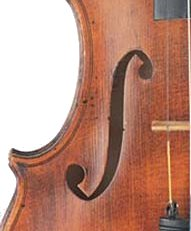
\includegraphics[width=4cm]{images/violin}


\column{0.55\textwidth}
\begin{block}{}
\begin{center}
\begin{large}
 \insertsubtitle
\end{large}

\vspace{.1cm}

\begin{Large}
\textbf{\inserttitle}
\end{Large}


\vspace{.3cm}

{\insertdate}

\end{center}
\end{block}
\end{columns}

}



\frame{
  \frametitle{Today...}

%\begin{columns}[c]
%\column{0.5\textwidth}
 \tableofcontents
%\column{0.5\textwidth}


Section 5.5 of Stewart has more examples.

%\end{columns}
}



\frame{
  \frametitle{But first...}


\begin{alertblock}{}

\begin{center}
{\Large Grouped Student Evaluation
\pause

~


of Teaching.}
\end{center}

\end{alertblock}

}
\frame{
  \frametitle{But first...}
\begin{alertblock}{}

\begin{center}
{\Large \Bf{REMINDER}\\
 Homework exercises from Problem Set 3 are due on
  Friday.
}
\end{center}
\end{alertblock}

Solutions must be carefully written and, if on more than one page,
stapled together. 


}


\section{Integration}
\frame{

In this section of the course, we are trying to solve problems of the
form
\begin{block}{}
Given a function \eq{f:\R \rightarrow \R}, find a function \eq{g} such
that \eq{g'(x) = f(x)}. That is, \alert{find the antiderivative of
  \eq{f}}.

\end{block}

Usually we will write it as \Emph{find the integral of \eq{f}}, i.e., 
\[
\text{ Evaluate } ~~ \I = \int f(x) dx.
\]


}


\subsection{The Mathematical Tables}

\frame{

For many fundamental functions we can simply lookup their 
antiderivatives  pages  41 and 42 of the Mathematical Tables.


}

\frame{
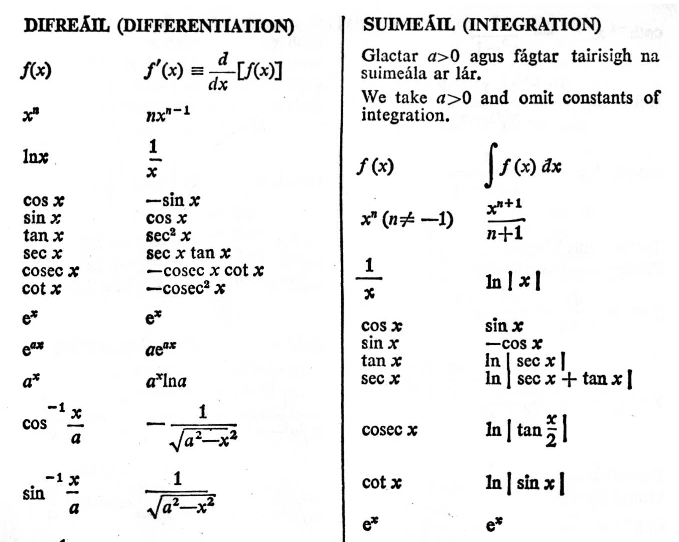
\includegraphics[width=10cm]{images/p41a}
}

\frame{

~


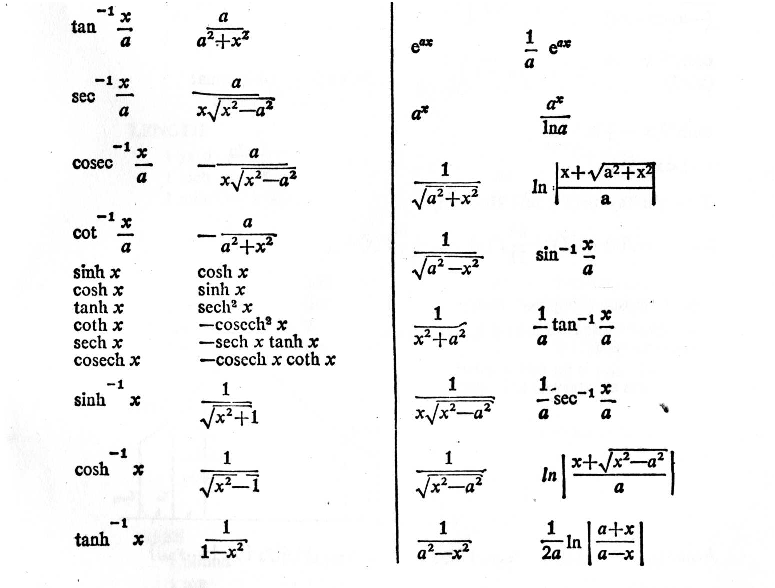
\includegraphics[width=10cm]{images/p41b}
}

\frame{
~

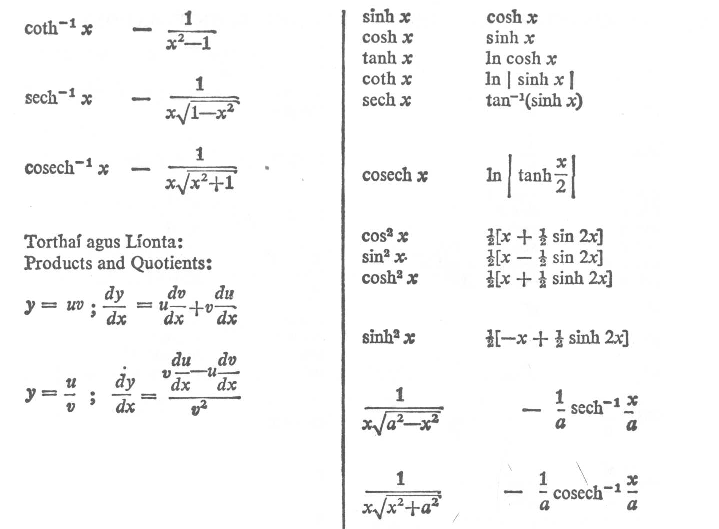
\includegraphics[width=10cm]{images/p42a}
}


\frame{

\begin{example}
Evaluate the following integral:
\eqd{ \int \tan^2 (x) dx.}
\end{example}
\vspace{4.5cm}
}



\frame{

In most cases, we can't just look-up the answer in a table.
We may have to simplify the express, e.g., using Partial Fractions, or
(more often) using a \Bf{Substitution}.

}

\section{Method of Substitution}

\frame{

\rblock
The method of substitution comes from the \Emph{Chain Rule of
  differentiation} and is summarised as

\begin{block}{Substitution}
Let \eq{u=g(x)}. The \eq{du = g'(x) dx}. So
\[
\int f'( g(x))g'(x) dx = \int f'(u)du = f(u) + C = f(g(x)) + C.
\]\end{block}

}

\subsection{Examples}


\frame{
\begin{example}
Evaluate the indefinite integrals\\
\[ 
(i) ~~ \alert{\mathcal{I}} = \int \sqrt{x+3}  dx. \pause
\qquad 
(ii) ~~ \alert{\I}= \int \frac{1}{\sqrt{x+3}}  dx.
\]
\end{example}

\vspace{5cm}

}


\frame{
\begin{example}
Evaluate the indefinite integral \quad \eqd{\alert{\I} = \int \frac{x}{x^2 +1} dx.}
\end{example}

\vspace{5cm}

}


\frame{
\begin{example}[Using Trigonometric Identities]
Evaluate the following integral:
\quad \eqd{ \alert{\I} = \int  \sec^4 (x) dx.}
\end{example}

\alert{Hint:} \eq{sec^2(x) = 1 + tan^2(x)}.

\vspace{4.5cm}
}






\frame{
\begin{example}
Evaluate the indefinite integral \eqd{ \I = \int \frac{\sin(3 \ln x)}{x} dx.}
\end{example}

\vspace{5cm}

}

\frame{
\begin{exercise}[17.1]
Evaluate the following integrals:
\begin{enumerate}[(i)]

\item \eqd{\int \frac{1+x}{\sqrt{1+x}} dx}.
\hspace{1.65cm}
(ii)~ \eqd{ \int  e^{(2x-2)} dx.}

\item[(iii)] \eqd{ \int  \frac{\sin(1/x)}{x^{2}} dx.}
\hspace{1.5cm}
(iv)~ \eqd{ \int e^{\sin(x)}\cos(x) dx}

\end{enumerate}
\end{exercise}

~


\begin{exercise}[17.2]
Use a suitable substitution to show that 
\[ \int \frac{1}{\tan(x)} dx = \ln |\sin(x)|.\]
\end{exercise}
\pause
\Emph{Hint:}

}



\subsection{Definite Integrals}
\frame{

\begin{block}{}
If \eq{g(a)=A} and \eq{f(b)=B} then 
\[
\int_a^b f\big( g(x) \big)g'(x) dx = \int_A^B f(u) du.
\]
\end{block}
\pause

\begin{example}
Evaluate 
\[ 
\int_0^8 \frac{ \cos\big(\sqrt{x+1}\big)}{\sqrt{x+1}} dx
\]
\end{example}
\vspace{2cm}
}


\frame{
\begin{exercise}[17.3]
Evaluate the following integrals:
\begin{enumerate}[(i)]
\item \eqd{ \int_0^4 \frac{x^3}{\sqrt{x^2 +1}} dx. }

\item \eqd{ \int_1^{\sqrt{e}}  \frac{ \sin\big(\pi \ln(x)\big)}{x} dx. } 

\item \eqd{\int_e^{e^2} \frac{1}{x \ln(x)} dx}.

\end{enumerate}
\end{exercise}

}


\subsection{Some more exercises}
\frame{

\begin{exercise}[17.4]
Evaluate the following integrals:
\begin{enumerate}[(i)]
\item  \eqd{\int x e^{x^2} dx}.
\item \eqd{\int \frac{\cos(x)}{4 + \sin^2(x)} dx.}

\item \eqd{\int e^{2x} \sin(e^{2x}) dx}

\item  \eqd{\int \frac{\ln(x)}{x} dx}

\item \eqd{ \int \frac{e^x+1}{e^x-1} dx}.

\end{enumerate}
\end{exercise}
}


\end{document}
